\documentclass[12pt]{article}
\usepackage[spanish]{babel}
\usepackage[utf8]{inputenc}
\usepackage[top=2.5cm,bottom=2.5cm,left=2.5cm,right=2.5cm]{geometry}
\usepackage{setspace}
\usepackage{graphicx}
\usepackage{pdfpages}

\begin{document}

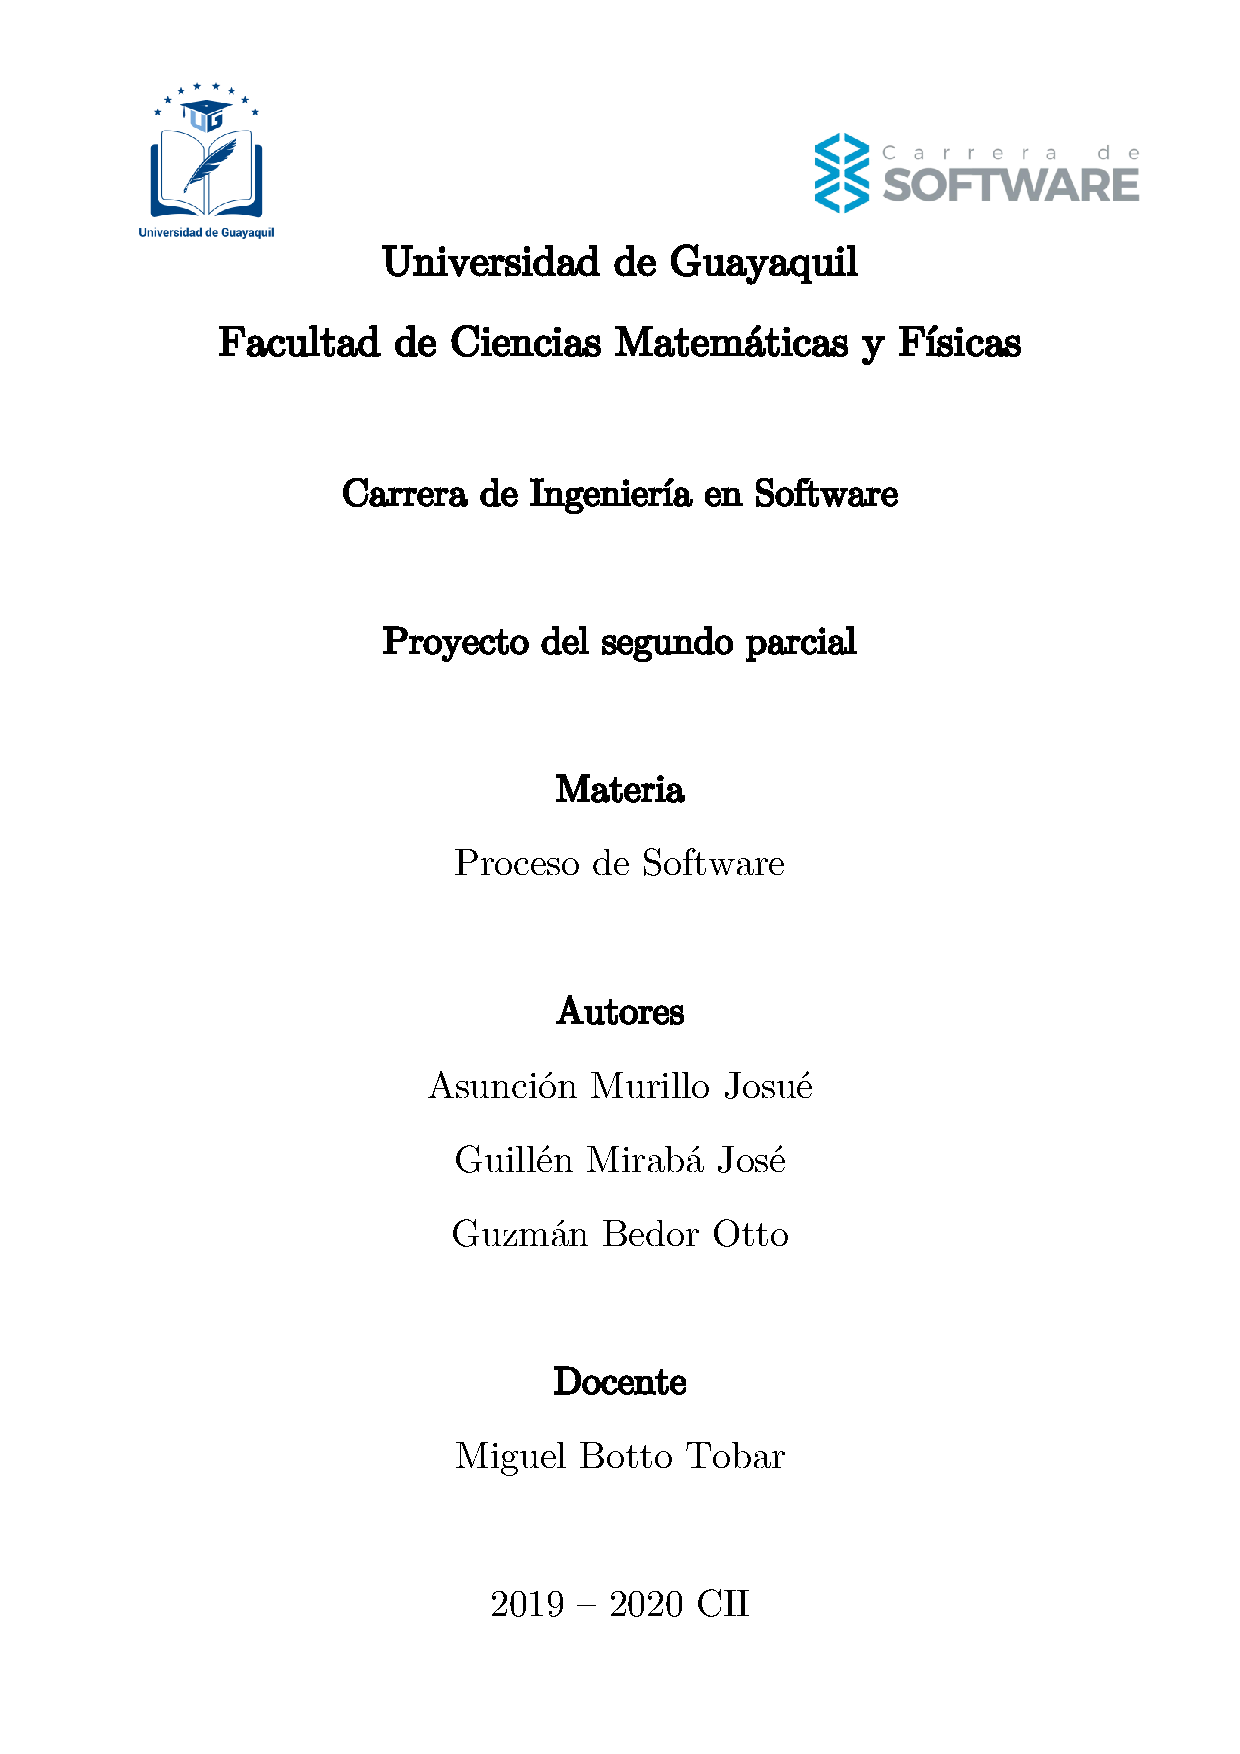
\includepdf{portada}

\doublespacing
\tableofcontents
\newpage


\section{Marco teórico}
La norma ISO 9001:2015 es una regla que estandariza el sistema de control de calidad de las organizaciones. ISO (Organización Internacional de Estandarización) es una entidad que reúne a representantes de diversos países para desarrollar normas de estandarización en diferentes áreas de actuación. La organización define normas para áreas como dimensión de papel, identificación de libros y grado de sensibilidad de películas fotográficas, tan sólo para citar algunas. En el caso de la norma ISO 9001, la más famosa de esas reglas, se trata de sistemas de gestión.

La sección que detalla la fase de ``diseño y desarrollo'' se encuentra en el punto 8.3 de la norma, y esta especifica que su aplicación no es obligatoria, puesto que solo es beneficiosa en empresas que crean un producto o servicio para posteriormente venderla, y no en una empresa que se dedique solo a comercializar productos realizados por otra empresa\\

\section{Norma ISO 9001:2015 aplicada en una empresa de desarrollo de software}     
\subsection{Caso de estudio}
La empresa TPV 123 desarrolló un software para mantener un control sobre el stock de productos por unidades vendidas, por materia utilizada en su elaboración, y control de todo tipo de ventas enfocadas en una panadería para facilitar estos procesos mediante sistemas digitales.\\

La planificación del diseño y desarrollo se realizó en cinco etapas:
\subsection{Planificación}
El programa está pensado para la satisfacción de una pequeña empresa de tipo panadería, la cual ayudará a mantener cierto grado de control sobre la producción y la venta, siendo este el modo de satisfacer los requisitos de la organización. Como exigencia legal, para el uso del programa debe quedar constancia de que la organización está debidamente registrada y legalizada, además de que debe contar con los respectivos permisos necesarios para laborar. A continuación se detallan algunos planteamientos del diseño del sistema:
\begin{itemize}
	\item Registro a los diferentes empleados que laboren en el establecimiento, quedando constancia de su respectivo y adecuado registro con la finalidad de llevar una mejor constancia de los mismos, haciendo uso de identificadores como la cédula o una foto.
	\item Un apartado de \textbf{mantenimiento}, en donde se puede hacer el registro de clientes, empleados, productos, proveedores, formas de pago.
	\item También consta con un apartado de \textbf{caja}, donde una nueva interfaz permite seleccionar qué empleado está haciendo uso del sistema en ese instante. La caja permite tener una previsualización de los productos en donde se podrá  seleccionar y hacer la contaduría de la venta, además permite seleccionar qué tipo de pago se realizará, y finalmente se podrá imprimir la factura respectiva.
	\item La opción de \textbf{listados}, permite generar informes de las diferentes funciones que realiza el programa como por ejemplo: un listado de empleados o clientes. Además permite una reimpresión de facturas y una caja diaria general.
	\item En el apartado de \textbf{stock}, se puede registrar productos recién ingresados y hacer un seguimiento regular del stock.
	\item La opción de \textbf{clientes con deuda} , permite tener un seguimiento de las ventas que no hayan sido canceladas completamente mediante el código de la factura, y el tipo de pago que fue seleccionado.
	\item El apartado de \textbf{promociones} , permite registrar productos con descuento, productos que vengan con un regalo, e incluso vales de descuento.
	\item La \textbf{agenda} , permite registrar citas entre los empleados y el encargado, con el fin de prestar ayuda a cualquier inconveniente.
	\item La opción de \textbf{estadísticas} , permite mostrar gráficos estadísticos de diversos aspectos como:  gráficos de ventas por empleado, por intervalos de tiempo y otros parámetros.
	\item El programa cuenta con una opción de \textbf{envío de email}, y además una opción de \textbf{control de horario}, que permite registrar la entrada y salida de los empleados al sistema.
	\item Con el fin de mantener una eficaz forma de comunicación con el usuario, se implementó una función de \textbf{asistencia} , que permite entre varias opciones elegir qué tipo de consulta se realizará, ademas que permite detallar qué tipo de problema se esta presentando, para que finalmente el usuario ingrese su correo y numero telefónico con los cuales empresa desarrolladora logrará ponerse en contacto directamente con el usuario, a fin de ayudar y satisfacer la necesidad presentada por alguna consulta relacionada al funcionamiento del sistema.
\end{itemize}

\begin{figure}[h]
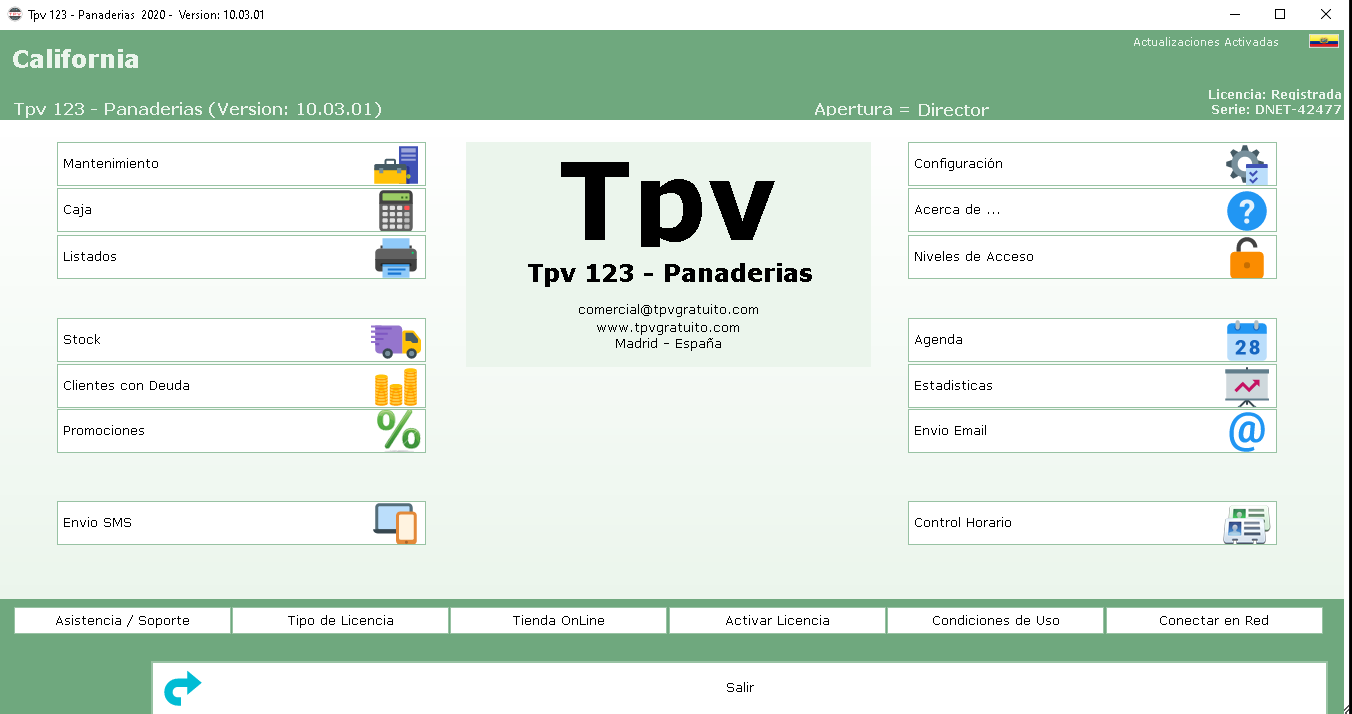
\includegraphics[scale=0.4]{interfaz.png}
\centering
\end{figure}


\subsection{Entradas para el diseño y desarrollo}
Las entradas para el diseño y desarrollo deben realizarse teniendo en cuenta los diferentes tipos de entradas para las funciones, a su vez debió pensarse cómo y para qué se tratará cada diferente tipo de dato respectivo a cada función. Teniendo eso en consideración, la revisión debió efectuarse con considerable éxito, además debieron derivarse nuevas ramificaciones o nuevos procesos y funciones, a fin de abarcar la mayor cantidad de resultados finales. El objetivo de esta etapa desde un principio se debió tratar con el único fin de tener consideraciones en el diseño del sistema, para que este sea accesible, agradable al cliente y que satisfaga la mayor cantidad de necesidades. 

El proceso para confirmar que las entradas operaban de forma correcta, fue mediante una revisión que se realizó a cada función por separado, teniendo en cuenta qué resultados se esperan, según qué tipo de datos se usan de entrada, por ejemplo, en el registro de empleados se buscaba guardar a cada empleado utilizando un identificador como la cédula, para tener control sobre quiénes están registrados, y si están legalmente ingresados el resultado esperado era el registro y guardado del empleado y su constancia dentro del sistema. También se utilizó una interacción entre el sistema y un usuario que realizara diferentes operaciones, para poder revisar el funcionamiento de una forma similar a como se espera que se realizará durante su uso una vez puesto en marcha.

Finalmente se debieron realizar pequeños cambios, con el fin de agregar funciones que al principio no estaban consideradas pero que a lo largo del diseño se debieron tomar en cuenta con el fin de ofrecer nuevas herramientas que servirán en otros ámbitos ya sean de toma de decisiones, manejo de inventarios o planificación laboral para los empleados, además de ofrecer una mejor capacidad de atención al cliente.

Aunque se ha detallado una pequeña parte de los controles del diseño y desarrollo, hacer esto fue necesario a fin de poder observar el comportamiento del sistema, en vista de que tiene sus diferentes funciones o procedimientos detallados de modo visible para el usuario, y confirmar que este a su vez respeta el diseño planteado anteriormente, y los resultados esperados sean correctos.

\subsection{Controles del diseño y desarrollo}
Como se expresó anteriormente, en la etapa anterior se logró observar que las funciones del sistema cumplen con sus respectivos procesos, es decir, cada función revisada ejecuta correctamente su labor dependiendo estrechamente de los requisitos planteados y de los datos ingresados o seleccionados, de tal modo que ninguna función entre en conflicto con otras o consigo misma, facilitando el correcto uso del sistema.

Principalmente esta etapa se realizó a manera de pruebas entre un usuario del sistema y un cliente, a modo de obtener diferentes resultados de acuerdo a lo que el cliente está deseando adquirir de los productos, así mismo como el registro tanto de empleados como de clientes y de visores estadísticos teniendo en cuenta una planificación previa de que tipo de resultados se esperaban que ocurrieran.

Se debió constar que algunas funciones están relacionadas con un personal que sirve como administrador, como por ejemplo el registro de empleados o la asignación de horarios, estás funciones también fueron revisadas y verificadas de forma sencilla siempre que se tuvieron a mano los datos solicitados. Para esta etapa se debió predefinir qué tipo de respuesta daría el sistema en relación a la interacción que el usuario daría, cumpliendo en cada validación el resultado esperado.

\subsection{Salidas del diseño y desarrollo}
Esta etapa busca asegurar que las salidas o resultados del sistema cumplan con los requisitos planteados en la planificación.

En nuestro caso el sistema es capaz de funcionar como un todo, de forma agradable al usuario y continua. Las diferentes funciones realizan sus cometidos sin generar errores y sin interponerse en el funcionamiento de otras, además de interactuar de forma sostenible entre ellas sin perder datos en el proceso.

En pocas palabras, el sistema es capaz de guiar de forma tácita al usuario, permitiendo tener una idea de qué realiza cada función planteada en el menú, solo guiándose con su nombre, y una vez que se hace uso de estas opciones, el usuario podrá manejarse con extrema simpleza a través de los diferentes campos, dado que el programa ofrece de forma visible una explicación de qué o cómo se esta llevando a cabo el procedimiento.

\subsection{Cambios al diseño y desarrollo}
En vista de que el desarrollo del sistema no fue realizado por nosotros, simplemente podemos entender de forma abstracta cómo se llevo a cabo, pero no podemos asegurar cómo o qué cambios fueron realizados a los largo del proceso, por ende solo podemos discernir que a fin de respetar y seguir la norma se debieron realizar diferentes documentaciones, en donde se especificaban qué cambios hubo y cómo afectaron estos cambios al sistema, además de que se debieron tomar medidas en caso de existir impactos adversos.

Sin embargo, nos es posible asegurar que en caso de que se realizaran cambios, estos generaron buenos resultados y permitieron conseguir un mejor sistema capaz de satisfacer las necesidades previamente dichas o aquellas que surgieron a lo largo del trabajo.

\newpage

\section{Conclusión}
El objetivo de este trabajo fue tener un entendimiento sobre cómo puede aplicarse la norma ISO 9001 en su versión 2015 a proyectos, trabajos o productos relacionados con el desarrollo de software, en nuestro caso y como se explicó al inicio del documento, el sistema que se utilizó es de acceso gratuito y desarrollado por una empresa desarrolladora de software TPV para diferentes tipos de negocios minoristas siendo el de nuestro ejemplo una panadería. 

Se debe recalcar que la ISO 9001 2015 especifica que las diferentes etapas detalladas en el diseño y desarrollo no son aplicables para todos los  proyectos con lo cual se debe considerar a qué tipo de proyecto se lo está considerando y qué tipo de enfoque se esta buscando.

A pesar de que se generó una pequeña documentación, es importante entender que entre mayor sea el producto o servicio, y mayor sea la capacidad de los desarrolladores, mayor será el tiempo necesitado para desarrollar una documentación que abarque todos los aspectos importantes del desarrollo de un software que permita satisfacer exitosamente una necesidad.
 
Finalmente cabe destacar que la norma aplicada para este trabajo solo es un estándar, y que puede ser seguido y desarrollado convirtiéndose en una norma  que explica el ``QUÉ'' se debe realizar, pero las empresas y los proyectos pueden ser complejos y está en manos de cada persona identificar ``CÓMO'' se llevara a cabo su desarrollo.

\newpage
\renewcommand{\refname}{Bibliografía}
\renewcommand{\bibname}{References}
\begin{thebibliography}{12}
	\bibitem{Martinez} Martínez, J. A. G. (2015). \emph{Guía para la aplicación de UNE-EN ISO 9001: 2015.} AENOR.
	\bibitem{Lopez} López Lemos, P. (2015). \emph{Cómo documentar un sistema de gestión de calidad según ISO 9001: 2015.} FC EDITORIAL.
\end{thebibliography}

\textbf{Dirección del repositorio de Github:}\\
https://github.com/JosueAsu/Proyecto-Procesos.git


\end{document}